\documentclass[11pt, letterpaper, twocolumn]{article}

% Input
\usepackage[english]{babel}
\usepackage[utf8]{inputenc}
% Geometry
\usepackage[margin=1.0in]{geometry}
\usepackage{titlesec}
\titleformat*{\section}{\large\bfseries}
\titleformat*{\subsection}{\bfseries}
% Fonts
%\usepackage{fontspec}
%xs\setmainfont{Arial}
% Figures and Symbols
\usepackage{graphicx}
\usepackage{caption}
\captionsetup[figure]{font=small}
\usepackage{amsmath}
\usepackage{amssymb}
\usepackage[]{siunitx}
% Misc
\usepackage{epigraph}
% Fancy Header
\usepackage{fancyhdr}
\setlength{\headheight}{14.5pt}
\pagestyle{fancy}
\fancyhf{}
% \renewcommand{\headrulewidth}{0pt}

\lhead{Fluid Simulation in CG WS2020 - RWTH Aachen } 
\rhead{Group 4: Ertural, Ledwon} 
\rfoot{\thepage}


\begin{document}
% Title, Abstract
\twocolumn[
\begin{@twocolumnfalse}
  \begin{center}
    \textbf{\large{Report: Fluid Simulation in Computer Graphics WS2020}}\\
    \vspace{0.1cm}
    \textbf{\small{Weakly Compressible Smoothed Particle Hydrodynamics
        \\and Position Based Fluids}}\\
    \vspace{0.2cm}
    \small{Berat Ertural, Dennis Ledwon\\
      RWTH Aachen, Visual Computing Institute\\
      Supervisor: Jose Antonio Fernandez Fernandez\\}

    \epigraph{Reading maketh a full man; conference a ready man; and writing an exact man.}
{\textit{Sir Francis Bacon}}
  \end{center}
\end{@twocolumnfalse}
]




\section{Introduction} \label{sec:introduction}

Fluids play a vital role in our lifes. Understanding the motion and behaviour of fluids is not only crucial to many fields of engineering, but it also aids us in creating beatiful virtual worlds, such as used in games and cinema. The simulation of fluids is a vast and rapidly growing field. During the course of this practical, we studied various methods, worked on simulations of our own and analysed different aspects a fluid solver.  

The motion of fluids is governed by the famous Navier-Stokes equation, as given below in its Lagrangian form;
\begin{equation}
  \dot{v}_i = \frac{\partial v_i}{\partial t} = -\frac{1}{\rho_i}\nabla p_i +\nu \nabla^2 v_i + \frac{F^{ext}_i}{m_i}.
\end{equation}
The Lagrangian form denotes the sampling points as dynamic particles moving with the flow of the fluid. The above PDE describes the acceleration \( \dot{v}_i\) of such a particle \( i \) as depending on the internal pressure gradient \( \nabla p_i\) and the veloctity divergence \( \nabla^2 v_i\) of the fluid. The velocity divergence and friction coefficient \( \nu \) represent the viscoscity of the fluid due to internal friction. The pressure gradient drives the acceleration due to internal pressure differences, to achieve incompressebility. In theory the density of the fluid is said to be constant, 
\(\frac{\delta \rho}{\delta t} = 0.\)
In practice, absolute incompressebility is not achievable due to numerical errors. Sometimes small deviations from the rest density of the fluid is desirable. This will be discussed in the next chapters. \cite{bender2015, ihmsen2014}

As with many PDE describing natural phenomena, the Navier-Stokes equation has no analytical solution. If it had, this report would end here with a reference to the proof of someone who is now one million dollars richer. Nonetheless, numerical approximations to fluid dynamics exist and during the course of the practical lecture we were tasked to implement two such solvers, namely Weakly Compressible Smoothed Particle Hydrodynamics (WCSPH) \cite{ihmsen2014} and Position based Fluids (PBF) \cite{macklin2013}. 
In the next section we will give a short overview of the used methods and implementation of the application.
We will then present various experiments and discuss our observations and the results.



\section{Methods} \label{sec:methods}
In the following a short overview of the methodological background and implementation will be given. In addition, certain aspects of the implementation that were done differently than from the given assignment will be presented.
For a thorough discussion of the SPH and PBF framework we refer the reader to the review of SPH fluids by Ihmsen et al. \cite{ihmsen2014} and to the original paper about PBF by Macklin et al. \cite{macklin2013}, as well as the works of Akinci et al. \cite{akinci2012, akinci2013}.

\subsection{Weakly Compressible SPH}
Smoothed Particle Hydrodynamics (SPH) is a class of particle based methods for fluid simulation with a long record of scientific publications.
The core idea of SPH is to approximate any attribute \( A_i\) of a point at an arbitrary position \(\vec{x}_i\) by weighting the attributes of the immediate surrounding particles \(j \in N \);
\begin{equation}
  A_i = \sum_{j \in N} \frac{m_j}{\rho_j}  A_j \cdot  W(||\vec{x}_i - \vec{x}_j||/h).
  \label{eq:weight}
\end{equation}
Particle mass \(m_j\) and density \(p_j\) is used as a normalization factor.
The weighting is performed by the so called kernel function \( W : \mathbb{R} \rightarrow \mathbb{R}\). It depends on the ratio of the distance between two particles and the smoothing length \(h\), which is defined to be a multiple of the particle diameter; \(h = \mu \cdot 2r\). We set \(\mu = 1.1.\) during the remainder of this report. The kernel is then given as \( W(q) = \frac{1}{h^3}f(q)\).
The function for the kernel used throughout the application is the following cubic spline \cite{monaghan1992},
\begin{equation}
  f(q) = \frac{3}{2\pi}
  \begin{cases}
    \frac{2}{3} - q^2 + \frac{1}{2}q^3 & 0 \leq q < 1 \\
    \frac{1}{6}(2-q)^3 & 1 \leq q < 2 \\
    0 & 2 \leq q \\
  \end{cases}
  .
\end{equation}
It should be noted, that the effective radius of the kernel function, and therefore the number of neighbourhood particles taken into account, depends on the smoothing length.
Weakly Compressible SPH first computes the particle density \(\rho_i\) using (\ref{eq:weight}) and then applies this to a so called Equation of State (EOS) to derive the resulting particle pressures \(p_i\). In the application the following EOS was used to derive the pressures;
\begin{equation}
  p_i = max(0, B(\rho_i - \rho_0)),
  \label{eq:pressure}
\end{equation}
where \(B\) is a stiffness constant. Equation (\ref{eq:pressure}) is similar to hookes law, as the pressure and therefore the resulting force depends linearly on the displacement. Therefore WCSPH allows for a small degree of incompressebility of the fluid. We will later discuss the implications of this. 
Using the formulations above we can derive expressions for the gradient and divergence field of an attribute and therefore compute the pressure and viscoscity term of the Navier-Stokes equation.

\subsection{Position Based Fluids}

Position Based Fluids (PBF) is a relatively new method based on the authors previous work on Position Based Dynamics (PBD) \cite{muller2007}.
Within this framework, a system is modelled using constraint functions, which describe the theoretical optimum or the equilibrium state. A solver will try to move the system towards the equilibrium by iteratively moving the positions of the sample points, such that the constraint violation is minimized. For fluidsimulations, PBF tries to achieve incompressibility by specifying the constraint (for a particle \(i\));
\begin{equation}
  C_i(\hat{x}) = \frac{\rho_i(\hat{x})}{\rho_0} - 1,
  \label{eg:pbfconstraint}
\end{equation}
where \(\hat{x}\) is the collection of all particles involved in the computation of \(\rho_i\). Therefore the solver will try to find a displacement \(\Delta \hat{x}\), such that \( C_i(\hat{x} + \Delta\hat{x}) = 0\). A sensible choice is to move the particles a fraction \(\lambda\) along the constraint gradient \(\nabla C\) proportional to inverse inertia \(M^{-1}\);
\begin{equation}
  \Delta\hat{x} = M^{-1} \nabla C \lambda.
  \label{eg:deltax}
\end{equation}
An approximate solution to the linear equation above is derived using a method similar to a Jacobi iteration. The velocities are then derived implicitly from the differences of the positions between frames.
In the application PBF is used to replace the computation of the pressure term in the Navier-Stokes equation. To avoid attractive forces, which may lead to particle clumping and unwanted behaviour, the constraint from (\ref{eg:pbfconstraint}) is changed to an inequality constraint, \(C_i > 0\).

\subsection{Neighborhood Search}
Most of the time the bottleneck of a particle based fluidsimulation is the neighborhood search.
An efficient algorithm to find the particles in direct proximity is key to a stable runtime performance. The application uses the CompactNSearch algorithm by Bender et al. \cite{bender2015}, which implements the parallel, hash-based neighborhood search by Ihmsen et al. \cite{ihmsen2011}. To further enhance runtime performance, we perform a Z-index sort of particle positions after a fixed number of iterations. Sorting the particles depending on their spatial properties will decrease the number of cache misses and therefore speed up the access time significantly.

\subsection{Time integration}
The system is advanced in time using the semi-implicit euler method, which is also known as the symplectic euler, as it conserves the energy over time.
Furthermore, XSPH smoothing is applied to the velocities.
The effect is that neighboring velocities are aligned towards each other, which results in a more viscous behaviour and helps to keep the simulation more stable.
The time step \(\Delta t\) is determined by the Courant-Friedrich-Levy (CFL) condition, \( \Delta t \leq \lambda \frac{2r}{||v_{max}||}\), with particle radius \(r\) and maximum particle velocity \(v_{max}\). The CFL condition sets the timestep dynamically, so that the particles will only move a fraction of their diameter during one iteration of the symplectic euler scheme. 
To further enhance the stability of the methods, we implemented a simple linear drag force which causes deaccalaration proportional to the velocity;
\begin{equation}
  f_{drag,i} = -k_{drag} \cdot v_i.
\end{equation}
The drag coefficient \(k_{drag}\) should ideally be below 0.1 as to not slow down the simulation too much. The implemented drag force is not ideal and in no way realistic. Modelling realistic drag for SPH methods with multiphase coupling and liquid-air interaction remains an active research field.

\subsection{Boundary Interaction}
To realise the interaction between the fluid and rigid boundaries, we use the boundary particle method by Akinci et al. \cite{akinci2012}. By taking advantage of the particle based nature of the presented methods we are able to integrate contributions from boundary particles into the calculations of densities, forces and position corrections.
Boundaries in a scene are usually represented by triangle mesh models. By sampling each surface triangle, we are able to sample the whole input mesh.
To this end is reasonable to dissolve a higher resolution mesh into a low resolution mesh which preserves the topological shape, use the low res mesh for the simulation and keep the original high resolution mesh for rendering the final simulation. This will reduce the overall number of triangles and therefore the number of sampled particles. Figure \ref{fig:mesh} shows and example of the armadillo mesh used for most simulations in this report.

\begin{figure}[ht]
    \centering
    \includegraphics[width=0.5\textwidth]{images/mesh.png}
    \caption{High resoltuion mesh for rendering (left) and low resolution mesh for simulation (right). The mesh on the left maintains the topological shape of the original.}
    \label{fig:mesh}
\end{figure}
To sample the particles on a triangle surface we perform a variation of the Pineda algorithm \cite{pineda1988} in the local coordinate system of the triangle surface.
% Given a triangle specified by the three vertex points \(a, b, c \in \mathbb{R}^3\), we construct the orthonormal base vectors \(u,v,n \in \mathbb{R}^3\) defining the triangle surface.
The basis transform that will yield the local triangle coordiantes \(p \in \mathbb{R}^2\) for a point in global space \(x \in \mathbb{R}^3\) is given in (\ref{eq:localtriangle}).
\begin{equation}
  p = 
  \begin{pmatrix}
    u_x & u_v & u_z & u^T a\\
    v_x & v_v & v_z & v^T a\\
    0 & 0 & 0 & 1 \\
  \end{pmatrix}
  \cdot x 
\label{eq:localtriangle}
\end{equation}
The orthonormal basis vectors of the triangle \(u, v \in \mathbb{R}^3\) are parallel to the plane. The basis vector perpendicular to the plane is not used. The origin of the local coordinate system is a triangle corner \(a \in \mathbb{R}^3\).
Applying the pineda algorithm is now straightforward. We first enclose the triangle by an axis-aligned bounding box (AABB) in the local coordiante system.
We then go along the bounding box and check for each sample point if its inside the triangle by checking against its edges, as described by Pineda \cite{pineda1988}.
We use a hexagonal sampling pattern to ensure maximum coverage of the surface. Figure \ref{fig:trianglesampling} demonstrates the hexagonal sampling in the bounds of the rectangle enclosing the triangle in its local coordinate system. Sample points inside the triangle are shaded opaque blue and sample points outside are transparent. The borders are slightly offset as to allow more samples to be inside the triangle. This is to ensure that the triangle mesh of the boundary has no holes where the edges of two triangles meet.
The oversampling is later compensated by recomputing the volume of each boundary particle depending on the number of particles in its close neighbourhood.

\begin{figure}[ht]
    \centering
    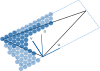
\includegraphics[width=0.4\textwidth]{images/triangle.pdf}
    \caption{Hexagonal sampling using pineda algorithm in local triangle space.}
    \label{fig:trianglesampling}
\end{figure}
We transform the sampled points back into three dimensional global space by multiplying them by the inverse of (\ref{eq:localtriangle}). Since the matrix is orthonormal its inverse is given by simply transposing the matrix.

\subsection{Tension and Adhesion}
Surface tension effects are implemented according the method by Akinci et al. \cite{akinci2013}.
Akinci et al. define two types of forces, namely fluid cohesion and boundary adhesion. Fluid cohesion is an attractive force between particles. Macroscopically, it acts as a force field around the surface of the fluid which keeps the particles together. In this way surface tensions is realised and effects such as waterdroplets become arise. The adhesion force causes fluid particles to stick to solid boundaries, which results in a wetting effect.

\subsection{Surface Reconstruction}
To extract an explicit representation of the fluid surface, a signed distance function (SDF) \(\Phi(\vec{x}) \) describing the isosurface is required. We use the SPH method to approximate the isosurface at any arbitrary point \(\vec{x}\), depending on the normalized density \(\rho_j\) of the neighborhood region \(j \in N\);
\begin{equation}
  \Phi(\vec{x})= \sum_{j \in N(\vec{x})}\frac{1}{\rho_j} W(||\vec{x} - x_j|| / h) - c.
\end{equation}
The parameter \(c\) controls the zero level of the isosurface and therefore the enclosed volume of the explicit representation. We set \(c = 0.6\) during the remainder of the report. Using this method, we compute \(\Phi(\vec{x})\) at points in a grid and extract the triangle mesh representing the surface according to the Marching Cubes algorithm \cite{lorensen1987}.

% marching cubes


\subsection{Implementation}
The implementation uses a primarily imperative programming style with the exception of a few object oriented paradigms. Data encapsulation in the form of C++ classes is applied to ensure data consistency during computation. Basic inheritance is used to be able to reuse code for different parts of the program. This style of programming allows us to be flexible enough to incrementially implement the practical assignment tasks while sacrificing little to no performance due to design overload.
\begin{figure}[ht]
    \centering
    \includegraphics[width=0.5\textwidth]{images/system.pdf}
    \caption{Schematic overview of the implementation.}
    \label{fig:systemuml}
\end{figure}
  
The implementation is divided into two broad categories, systems and solvers.
What we define as a system, includes fluid- and boundaryparticles, their generalization as particlesystems and auxilary constructs concerning particles. These represent the creation, state and behaviour of fluid- and boundary particles.
On the other hand, we have two seperate specific solvers for WCSPH and PBF. They aggregate fluid- and boundarysystems to model the progression of the given system. The specific solvers share a some functions and general parameters over their superclass. Since the function that starts a simulation run is defined over the superclass, it is possible to determine the type of solver at runtime.
Figure \ref{fig:systemuml} gives a schematic UML diagram of the relation between the different parts of the implementation.
A particlesystem is a collection of particles which are represented by basic attributes, such as mass, density, position, velocity, etc. Since it is vital to keep all attributes of a particlesystem consistent during computation, a particlesystem object is only allowed to be created by the emitter object. The emitter object is a singleton, which means that there is always one and only one single instance of the object during the runtime of the program. A particlesystem is present in two forms, either as fluid particles or as boundary particles. These subtypes posess attributes and methods responsible for the behaviour of fluid or boundary particles in a system. For example, boundary particles possess a seperate variable volume attribute and a method to compute the volume for each particle depending on the density, e.g. the number of boundary particles in close neighbourhood. All particlesystems make use of precomputed lookup tables of the kernels. Since the kernel is evaluated a large number of times per particle, the lookup tables provide a significant speedup.
In addition, each solver has been parallelized using OpenMP. To reduce the overhead from excessive creation and deletion of threads, a parallel region is created once upon entering an integration step. In this case special care has to be taken to avoid race conditions due to shared memory between threads. 

\section*{Results}
\label{sec:results}


\section*{Conclusion}
\label{sec:conclusion}

% respong to introduction and discuss implications of result


\section*{Outlook}
\label{sec:future}
The WCSPH and PBF implementation as well as the surface reconstruction offers a high level of concurency in the form of data parallelism. This means, that there are many parts in the programm where sequentially processed data can be split into independant groups which can be processed in parallel.

% what are the next steps?
% what did we learn from this and how could we apply this for the future?



\bibliographystyle{alpha}
{\footnotesize
\bibliography{references.bib}}


% tables, if needed, are like this.
% \begin{table}[ht]
% \begin{tabular}{|l|l|l|}
% \hline
% Time (s) & Distance (m) & Charge (C) \\ \hline
% 0        & 0            & 10         \\ \hline
% 1        & 1            & 5          \\ \hline
% 2        & 4            & 6          \\ \hline
% \end{tabular}
% \caption{An example table.}
% \label{table:ExampleTable}
% \end{table}

% \begin{figure}[ht]
%     \centering
%     \includegraphics[width=0.5\textwidth]{img/generic_plot.pdf}
%     \caption{Here is a caption for a figure.}
%     \label{fig:ExampleFigure}
% \end{figure}

\end{document}

%%% Local Variables:
%%% mode: latex
%%% TeX-master: t
%%% End:
